\chapter{Setting Up the Project}

\section{Hardware Setup}

For a guide on how to connect the hardware, consult figure \ref{fig:power} and \ref{fig:sensor_connections}. Otherwise, see the hardware list. A principal connection diagram for the network is shown in figure \ref{fig:network_setup}. The router should already be configured for communications. If not, consult \cite{aspunvik}.

\begin{figure}[h]
	\centering
	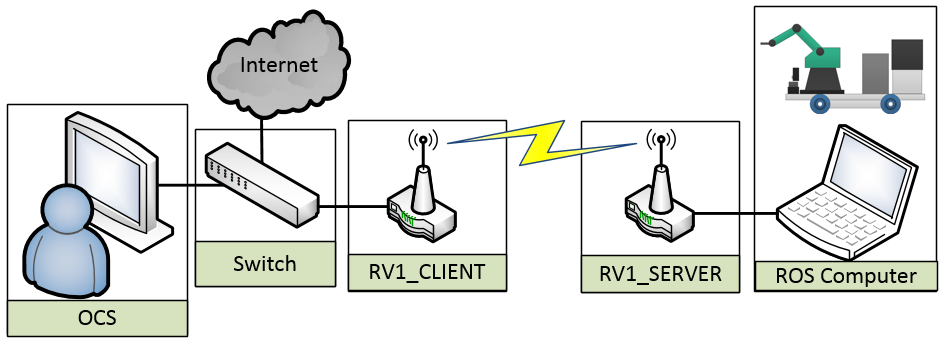
\includegraphics[width=0.85\textwidth]{network_setup}
	\caption{Network hardware setup. }
	\label{fig:network_setup}
\end{figure}

\subsubsection{Lead Battery Safety Precautions}

The lead battery used in this project (black 24V 48Ah, Biltema), contains a large amount of energy and highly corrosive sulfuric acid. Remember to read the warning label on the battery, and handle the battery with care. 

An explosive mix of hydrogen and oxygen may be formed when charging the battery. Some safety precautions are necessary to handle the risk:

\begin{itemize}
	\item Always charge the battery in a well ventilated area. 
	\item Turn the charger off before removing the connecting clamps.
	\item Allow some time to pass after charging before connecting or disconnecting cables to the battery poles.
\end{itemize} 

\subsubsection{Equipment List}
\begin{itemize}
	\item A computer that can be mounted on the robot. The computer must run on Linux Ubuntu (13.10 or 14.04 for ROS Indigo) and have a Bluetooth adapter.
	\item Two wireless routers (for example TP-Link).
	\item Two sinus inverters. One power inverter from Biltema and a silver colored pure sine inverter.
	\item One 12V Battery. The battery used in this project has a capacity of $45 Ah$.
	\item A $230V AC/24V DC$ converter.
	\item One XMEGA A3BU evalation board.
	\item One Hokuyo URG-04LX-UG01 LIDAR.
	\item A Kinect for XBOX 360 or an equivalent OpenNI depth camera.
\end{itemize}



\section{Installation}

\subsection{Software list}

This guide assumes that ROS Indigo is being used on a comparable system, for example Ubuntu 14.04. A guide for installing either ROS or Ubuntu is best aquired elsewhere. For ROS, see \url{ros.org}. Indigo was chosen primarily because of \texttt{openni\_launch}. 

\begin{description}
	\item[Hector SLAM for ROS] Install with \begin{verbatim} sudo apt-get install ros-indigo-hector-slam \end{verbatim}
	\item[Web video server node] Install with \begin{verbatim} sudo apt-get install ros-indigo-web-video-server \end{verbatim}
	\item[LIDAR driver] Install with \begin{verbatim} sudo apt-get install ros-indigo-hokuyo-node \end{verbatim}
	\item[RTAB-Map] Installed from source. Guide available at\\
	\url{https://github.com/introlab/rtabmap/wiki/Installation#ros}
	\item[Gazebo]  Install with \begin{verbatim} sudo apt-get install ros-indigo-gazebo-ros-pkgs \end{verbatim}
	Otherwise, consult \url{http://wiki.ros.org/gazebo_ros_pkgs}.
\end{description}

\section{Configuring the Project}

\subsection{Configuring the ROS Workspace}

Assuming that ROS is installed and properly configured, the first step in configuring the project is to create a catkin workspace. The custom ROS packages bundled with the digital attachments, should be placed in the \texttt{src} folder within the catkin workspace.

\subsection{Configuring the Bluetooth Connection}

The Qt framework is used to simplify the implementation of the Bluetooth connection between the \ac{ROS} graph and a remote device. Our \ac{ROS} installation for this project already includes some variant of Qt version 4.8. While useful for creating new \ac{GUI} applications, it lacks a Bluetooth API. The latest version of Qt, version 5.x, is equipped with libraries necessary for developing Bluetooth applications. This part of the guide will explain how to create a Qt 5 application which can be build by \texttt{catkin\_make} and run as a \textit{rosnode}.

\subsubsection{1 - Install Qt5}

Installing Qt5 for Linux is a straight forward procedure. Go to \url{qt.io}, and download the free version of Qt. All necessary instructions are provided. Qt5 may be installed in the home folder.

\subsubsection{2- Enabling Qt5 in a ROS node}

It is assumed that the \ac{ROS} package \texttt{bluetooth\_server}, is located in a catkin workspace:
\begin{verbatim}
	<NAME OF CATKIN WORKSPACE>/src/bluetooth_server
\end{verbatim}

Inside this folder, open the file ''CMakeLists.txt'' and locate the following:

\begin{verbatim}
set(CMAKE_PREFIX_PATH "/home/vegard/Qt/5.5/gcc_64/lib/cmake/Qt5"
					  "/home/vegard/Qt/5.5/gcc_64/lib/cmake/Qt5Core"
					  "/home/vegard/Qt/5.5/gcc_64/lib/cmake/Qt5Bluetooth"
\end{verbatim}

Change these paths to the correct paths on your system.

% FJERN DETTE DELKAPITTELET!
%\subsection{Adding the Qwt Plugin For Customizing QDial}

%This is a ''howto'' guide on how to install the Qwt-plugin.The following is assumed:

%\begin{itemize}
%	\item Development is performed on Windows 7
%	\item Qt 5.x is installed at c:/Qt
%\end{itemize}

\section{System Launch Procedure}

This procedure assumes that the \ac{ROS} implementation source code is placed in the \texttt{src} folder of a catkin workspace, and that he project has been built successfully. The first step is to go through a hardware checklist:

\begin{enumerate}
	\item Verify that the motor control board is connected to the wheel drivers, as shown in figure \ref{fig:conn_diag_motors}.
	\item Kinect, router and motors are connected to either internal or external power.
	\item Ensure that all USB ports are free. Exceptions apply to devices such as the Kinect or a mouse. 
	\item Connect the Hokuyo lidar (URG-04LX-UG01) to a USB port.
	\item Connect the motor control card to a USB port. Ensure that it is connected after the LIDAR. Ensure that the correct firmware is installed on the board.
\end{enumerate}

This procedure is recorded to video ''start\_live\_robot'': 

\begin{enumerate}
	\item Open five terminal windows.
	\item Launch \texttt{roscore} in one of the windows
	\item \texttt{cd} to \texttt{<your\_catkin\_workspace>/src/mar/scripts>}
	\item In this folder, run \texttt{\$ sudo ./setup\_hokuyo.sh}
	\item In the remaining three terminals, \texttt{cd} to your catkin workspace.
	\item In each of the terminals, run \texttt{\$ source ./devel/setup.bash}
	\item In one terminal, bring up the robot with\\ \texttt{\$ roslaunch mar mar\_bringup.launch}
	\item In another terminal, launch rtabmap with\\ \texttt{\$ roslaunch mar rtabmap.launch}\\
	Consult the launch file to see argument options.
	\item In the last terminal, launch navigation with\\ \texttt{\$ roslaunch mar\_2dnav move\_base.launch}
\end{enumerate}

\chapter{Robot Mass Calculations}
\label{chp:mass}
\begin{verbatim}
	Mass density, Aluminium: 2,7 g/cm³
	
	----- Plate: -----
	
	Volume: 37x80x0,5 cm³ = 1480 cm³
	Mass: 1480 cm³ x 2,7 g/cm³ = 4 kg
	
	----- Bottom: ----- 
	
	Volume:  Four side plates:  2 x 40 x 5 x 0,2 cm³ = 160 cm³
	Aft and front:  2 x 36 x 5 x 0,2 cm³ = 72 cm³
	Miscellanious :	4*70 = 280 cm³
	
	Total: 440cm³
	
	Mass:   Aluminium: 440 cm³ * 2,7g/cm³ = 1188 g = 1,2 kg
	
	
	Wheel:	reference: 
	http://www.superdroidrobots.com/shop/item.aspx/omni-wheel-and-shaft
	-assembly-double-row/383/
	
	Mass m. shaft: 1,8 lbs = 816 g	
	
	Total mass, wheels: 4*816g = 3264 g = 3,3 kg 
	
	
	
	
	----- Arm: -----
	
	Robot arm:	reference: http://www.intelitek.com/robots/scorbot-er-4u/
	Controller reference: http://www.intelitek.com/robots/usb-controller/
	
	Robot arm mass: 10,8 kg
	Robot controller mass: 7 kg
	
	----- Rear compartment (rack): -----
	
	Guessing at 20 kg (battery, computers, chassis etc.)
	l_x = 35 cm
	l_y = 37 cm
	l_z = 40 cm
\end{verbatim}